\chapter{Аналитический раздел}
В данном разделе будут рассмотрены теоретически основы работы алгоритма свёртки и основные принципы параллельного программирования.

\section{Алгоритм свёртки}
Алгоритм свёртки является реализацией операцией свёртки, которая используется в свёрточных нейронных сетях. Данный вид нейросетей обрабатывает изображения, которые подаются на вход алгоритму в виде матрицы пикселей. Операция свёртки позволяет находить и максимизировать признаки по которым нейросеть осуществляет какие-либо действия с алгоритмом.

Алгоритм свёртки работает следующим образом:
На вход алгоритма подаётся некая матрица A размера M x N. За тем к каждому элементу матрицы применяется ядро, представляющее из себя матрицу небольших размеров. В нашем случае будет использоваться матрица размером 3 на 3, выглядящая следующим образом:

\begin{equation}
	K = \left(
	\begin{array}{ccc}
			0 & -1 & 0\\
			-1 & 5 & -1\\
			0 & -1 & 0\\
		\end{array}
	\right)
\end{equation}

Для каждой области 3 на 3 в матрице применяется данный фильтр. Новое значение вычисляется путём суммирования произведений наложившихся элементов. Результат записывается в новую матрицу, размерности которой уменьшается на два.

\begin{figure}[ph!]
	\center{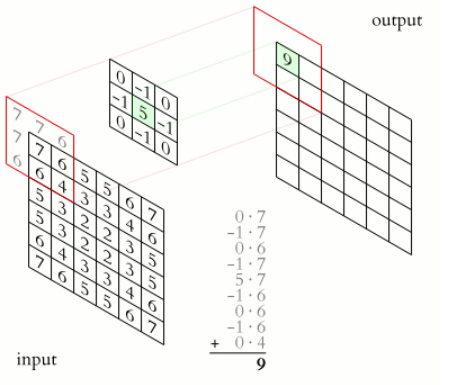
\includegraphics[scale=0.8]{conv_explain}}
	\caption{Схема работы операции свёртки}
\end{figure}

\newpage

\section{Параллельный алгоритм свёртки}
Так как каждая операция применения ядра происходит независимо от друг друга, мы можем выполнять их параллельно. В нашем случае мы будем выполнять их параллельно для каждого ряда матрицы. То есть например если у нас есть два потока, то первый параллельно посчитает чётные ряды, а второй нечётные.

\section{Параллельное программирование}
При использовании многопроцессорных вычислительных систем с общей памятью обычно предполагается, что имеющиеся в составе системы
процессоры обладают равной производительностью, являются равноправными при доступе к общей памяти, и время доступа к памяти одинаково (при одновременном доступе нескольких процессоров к одному и тому же элементу памяти очередность и синхронизация доступа обеспечивается на аппаратном уровне). Многопроцессорные системы подобного типа обычно именуются симметричными мультипроцессорами. Перечисленному выше набору предположений удовлетворяют также активно развиваемые в последнее время многоядерные процессоры, в которых каждое ядро представляет практически независимо функционирующее вычислительное устройство. Обычный подход при организации вычислений для многопроцессорных вычислительных систем с общей памятью — создание новых параллельных методов на основе обычных последовательных программ, в которых или автоматически компилятором, или непосредственно программистом выделяются участки независимых друг от друга вычислений. Возможности автоматического анализа программ для порождения параллельных вычислений достаточно ограничены, и второй подход является преобладающим. При этом для разработки параллельных программ могут применятся как новые алгоритмические языки, ориентированные на параллельное программирование, так и уже имеющиеся языки, расширенные некоторым набором операторов для параллельных вычислений.[1]

\section{Вывод}
В данном разделе были рассмотрены основные теоретические сведения об алгоритме свёртки и параллельном алгоритме свёртки. В результате были сделаны выводы о том, что на вход алгоритму подаётся матрица произвольных размеров, на выходе программа возвращает новую матрицу, полученную путём применения фильтра к старой. Алгоритмы работают на матрицах с размерностями от 3 до физически возможного предела для изпользуемой машины. В качестве критерия для сравнения эффективности алгоритмов будет использоваться время работы на матрицах различного размера.

\chapter{Конструкторский раздел}

В данном разделе будут рассмотрены схемы, структуры данных, способы тестирования, описания памяти для следующих алгоритмов:
\begin{enumerate}
	\item алгоритм свёртки;
	\item параллельный алгоритм свёртки.
\end{enumerate}

\section{Тестирование алгоритмов}

Описание классов эквивалентности:
\begin{enumerate}
	\item проверка работы на общем случае.
\end{enumerate}

Описание тестов:
\begin{enumerate}
	\item тест на общем случае - на вход подаётся матрица размерами m на n, выход сравнивается с заранее известным правильным результатом.
\end{enumerate}

\section{Алгоритм свёртки}

Используемые типы и структуры данных включают в себя:
\begin{enumerate}
	\item integer, целое число - используется для хранения индексов массива, размера массива;
	\item array, массив целых чисел - используется для хранения серии целых чисел;
	\item matrix, массив массивов целых числел - представление матрицы в программе.
\end{enumerate}

\newpage

\begin{figure}[ph!]
	\center{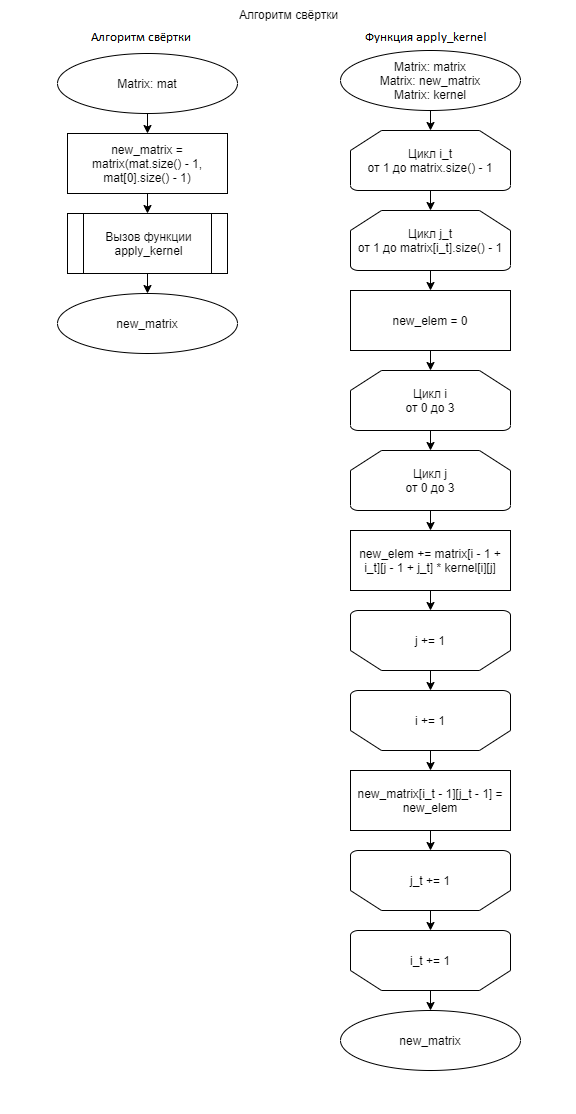
\includegraphics[scale=0.8]{conv_scheme}}
	\caption{Схема алгоритма свёртки}
\end{figure}

\section{Параллельный алгоритм свёртки}

Используемые типы и структуры данных включают в себя:
\begin{enumerate}
	\item integer, целое число - используется для хранения индексов массива, размера массива;
	\item array, массив целых чисел - используется для хранения серии целых чисел;
	\item matrix, массив массивов целых числел - представление матрицы в программе;
	\item vector, вектор - вид связного списка, позволяющий осуществять доступ к элементам по индексу.
\end{enumerate}

\begin{figure}[ph!]
	\center{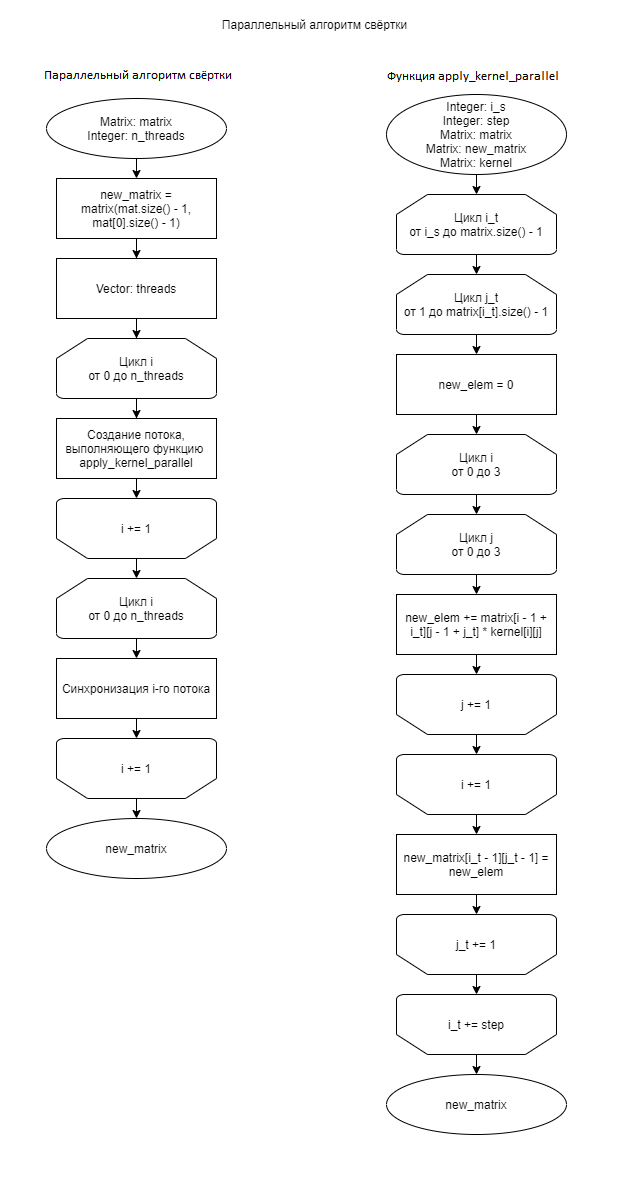
\includegraphics[scale=0.8]{conv_parallel_scheme}}
	\caption{Схема параллельного алгоритма свёртки}
\end{figure}

\section{Функциональная схема ПО}
На изображении ниже представлена функиональная схема разрабатываемого ПО. На вход подаётся матрица, заполненная целыми числами и при помощи алгоритмов, реализованных на языке С++ мы получаем в результате работы новую матрицу, содерждащую в себе результат свёртки.

\begin{figure}[ph!]
	\center{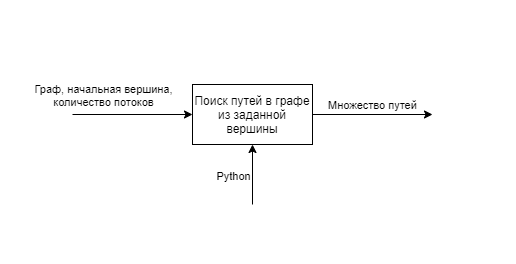
\includegraphics[scale=1.0]{func_scheme}}
	\caption{IDEF0 диаграмма разрабатываемой программы}
\end{figure}

\section{Вывод}
В данном разделе были рассмотрены схемы алгоритмов для параллельного не обычного алгоритма свёртки, и были определены тесты для каждого алгоритма, были описаны типы и структуры данных, использующихся в алгоритмах. Также была приведена функциональная схема разрабатываемого ПО.

\chapter{Технологический раздел}

В данном разделе будут рассмотрены подробности реализации описаных выше алгоритмов. Также будут обоснованы выбор языка программирования для реализации, выбор библиотек для проведения экспериментов и представлены важные фрагменты кода написанной в рамках работы программы.

\section{Выбор языка программирования}

В качестве языка программирования для реализации данной лабораторной работы использовался язык программирования C++ поскольку в данном языке есть стандартная библиотека thread в которой реализованы основные методы для работы с потоками. В качестве среды разработки использовалась Microsoft Visual Studio 2019 по причине того, что данная среда имеет встроенные средства отладки и анализа программ.

\section{Сведения о модулях программы}

Реализованное ПО состоит из трёх модулей:
\begin{enumerate}
	\item Convolutionizer - в данном модуле реализованы алгоритмы свёртки;
	\item lab\_4 - основной файл программы, где находится точка входа;
	\item tests - реализация тестов алгоритма;
	\item time - реализация замеров времени работы программы.
\end{enumerate}

\section{Реализация алгоритма свёртки}

\begin{lstlisting}[label=some-code-1,caption=Реализация алгоритма свёртки в виде метода класса Convolutionizer]
std::vector<std::vector<int>> Convolutionizer::convolution(std::vector<std::vector<int>> matrix)
{
	std::vector<std::vector<int>> new_matrix(matrix.size() - 2, std::vector<int>(matrix[0].size() - 2, 0));

	apply_kernel(matrix, new_matrix);
	return new_matrix;
}
\end{lstlisting}


\begin{lstlisting}[label=some-code-2,caption=Реализация функции применения ядра к матрице]
void Convolutionizer::apply_kernel(std::vector<std::vector<int>>& matrix, std::vector<std::vector<int>>& new_matrix)
{
	for (int i_t = 1; i_t < matrix.size() - 1; i_t++)
	{
		for (int j_t = 1; j_t < matrix[i_t].size() - 1; j_t++)
		{
			int new_elem = 0;
			for (int i = 0; i < 3; i++)
			{
				for (int j = 0; j < 3; j++)
				{
					new_elem += matrix[i - 1 + i_t][j - 1 + j_t] * kernel[i][j];
				}
			}
			new_matrix[i_t - 1][j_t - 1] = new_elem;
		}
	}
}
\end{lstlisting}

\section{Реализация параллельного алгоритма свёртки}

\begin{lstlisting}[label=some-code-3,caption=Реализация параллельного алгоритма свёртки в виде метода класса Convolutionizer]
std::vector<std::vector<int>> Convolutionizer::convolution_parallel(std::vector<std::vector<int>> matrix, int n_threads)
{
	std::vector<std::vector<int>> new_matrix(matrix.size() - 2, std::vector<int>(matrix[0].size() - 2, 0));

	std::vector<std::thread> threads;

	for (int i = 1; i <= n_threads; i++)
	{
		threads.push_back(std::thread(apply_kernel_parallel, i, n_threads, std::ref(matrix), std::ref(new_matrix), std::ref(kernel)));
	}

	for (auto& thread : threads)
		thread.join();
	threads.clear();


	return new_matrix;
}
\end{lstlisting}


\begin{lstlisting}[label=some-code-4,caption=Реализация функции применения ядра к матрице]
void apply_kernel_parallel(int i_s, int step, std::vector<std::vector<int>>& matrix, std::vector<std::vector<int>>& new_matrix, std::vector<std::vector<int>>& kernel)
{
	for (int i_t = i_s; i_t < matrix.size() - 1; i_t += step)
	{
		for (int j_t = 1; j_t < matrix[i_t].size() - 1; j_t++)
		{
			int new_elem = 0;
			for (int i = 0; i < 3; i++)
			{
				for (int j = 0; j < 3; j++)
				{
					new_elem += matrix[i - 1 + i_t][j - 1 + j_t] * kernel[i][j];
				}
			}
			new_matrix[i_t - 1][j_t - 1] = new_elem;
		}
	}
}
\end{lstlisting}

\section{Реализация тестирования алгоритмов}

Для тестирования алгоритмов было реализованы следующие тесты:
\begin{enumerate}
	\item тест на свёртку матрицы 5 на 5, заполненной заранее известными значениями;
\end{enumerate}

\begin{lstlisting}[label=some-code-7,caption=Реализация тестов]      
void test()
{
	Convolutionizer conv;
	std::vector<std::vector<int>> matrix(5, std::vector<int>(5, 0));

	for (int i = 0; i < 5; i++)
	{
		for (int j = 0; j < 5; j++)
		{
			if (i == j)
				matrix[i][j] = i + j;
		}
	}

	std::vector<std::vector<int>> correct_result = {
		{10, -6, 0},
		{-6, 20, -10},
		{0, -10, 30}
	};

	std::vector<std::vector<int>> result;
	bool flag;

	result = conv.convolution(matrix);
	flag = true;
	for (int i = 0; i < 3; i++)
	{
		for (int j = 0; j < 3; j++)
		{
			if (result[i][j] != correct_result[i][j])
				flag = false;
		}
	}
	std::cout << "TEST CONV SIMPLE: " << flag << std::endl;

	result = conv.convolution_parallel(matrix, 1);
	flag = true;
	for (int i = 0; i < 3; i++)
	{
		for (int j = 0; j < 3; j++)
		{
			if (result[i][j] != correct_result[i][j])
				flag = false;
		}
	}
	std::cout << "TEST CONV PARALLEL 1: " << flag << std::endl;

	result = conv.convolution_parallel(matrix, 2);
	flag = true;
	for (int i = 0; i < 3; i++)
	{
		for (int j = 0; j < 3; j++)
		{
			if (result[i][j] != correct_result[i][j])
				flag = false;
		}
	}
	std::cout << "TEST CONV PARALLEL 2: " << flag << std::endl;

	result = conv.convolution_parallel(matrix, 3);
	flag = true;
	for (int i = 0; i < 3; i++)
	{
		for (int j = 0; j < 3; j++)
		{
			if (result[i][j] != correct_result[i][j])
				flag = false;
		}
	}
	std::cout << "TEST CONV PARALLEL 3: " << flag << std::endl;

	result = conv.convolution_parallel(matrix, 4);
	flag = true;
	for (int i = 0; i < 3; i++)
	{
		for (int j = 0; j < 3; j++)
		{
			if (result[i][j] != correct_result[i][j])
				flag = false;
		}
	}
	std::cout << "TEST CONV PARALLEL 4: " << flag << std::endl;
}
\end{lstlisting}

\section{Вывод}
В данной разделе были представлены реализации алгоритма свёртки и параллельного алгоритма свёртки и показана реализация модуля тестирования реализованных алгоритмов.

\chapter{Экспериментальный раздел}

В данном разделе будут измерены временные характеристики алгоритмов свёртки и сделаны выводы об эффективности применения параллельного программирования для улучшения временных показателей данного алгоритма.

\section{Технические характеристики}
\begin{itemize}
	\item Операционная система - Windows 10, 64-bit;
	\item Оперативная память - 16 GiB;
	\item Процессор - Intel(R) Core(TM) i7-9750H CPU @ 2.60GHz 2.59 GHz, 6 ядер, 12 потоков.
\end{itemize}

\section{Результаты экспериментов}

\begin{table}[h!]
  \begin{center}
    \captionsetup{justification=raggedright}
    \caption{Время работы алгоритмов}
    \label{tab:workcost_classic}
    \begin{tabular}{c|c|c|c|c|c|c|c|c}
      \textbf{разм.} & \textbf{без параллел.} & \textbf{1 пот.}  & \textbf{2 пот.}  & \textbf{4 пот.}  & \textbf{8 пот.}  & \textbf{16 пот.}  & \textbf{32 пот.}  & \textbf{64 пот.}\\
      \hline
	100 & 124254 & 197843 & 91950 & 107883 & 113683 & 203370 & 362230 & 757957\\
	200 & 571961 & 483974 & 262076 & 201323 & 267745 & 246797 & 405434 & 950245\\
	300 & 1009692 & 1160469 & 626281 & 491241 & 336894 & 460936 & 843504 & 1615922\\
	400 & 2087216 & 1783830 & 1068245 & 674139 & 486513 & 705944 & 729709 & 914305\\
	500 & 3712886 & 3566122 & 1674925 & 937623 & 695409 & 779717 & 922891 & 1271875\\
	600 & 3526846 & 3513634 & 1853524 & 1135061 & 926665 & 940431 & 1123670 & 1538386\\
	700 & 4656533 & 5051931 & 2739630 & 1797084 & 1148615 & 1206905 & 1160595 & 1459891\\
	800 & 6670162 & 6919744 & 3299232 & 2074498 & 1539406 & 1587812 & 1466115 & 1668359\\
	900 & 8162026 & 8338385 & 5350798 & 3396232 & 2092533 & 2134784 & 1708677 & 2034956\\
	1000 & 10883751 & 10330769 & 5161384 & 3280373 & 2272809 & 2155541 & 2157472 & 2421776\\
	1100 & 13378364 & 12503826 & 6754120 & 4009432 & 2722892 & 2562020 & 2667564 & 2683358\\
	1200 & 15948354 & 14565637 & 8896638 & 5309428 & 3196955 & 3128936 & 3634144 & 3008889\\
	1300 & 17172619 & 15685027 & 8315751 & 5159352 & 3544501 & 3480708 & 3510173 & 3690841\\
	1400 & 21081695 & 19692531 & 11316242 & 6189062 & 4332132 & 4140771 & 3902364 & 4147262\\
	1500 & 22604317 & 22169477 & 11080092 & 7004708 & 4790231 & 4193591 & 4256824 & 4322949\\
	1600 & 25236594 & 26698045 & 14522262 & 8164930 & 5754227 & 4816110 & 4985526 & 5676034\\
	1700 & 30790852 & 28845662 & 16219230 & 10956174 & 6725419 & 5805027 & 5550661 & 6287667\\
	1800 & 36404743 & 33998653 & 18231903 & 9364057 & 6975351 & 5999613 & 6481451 & 6443922\\
	1900 & 38265471 & 37343315 & 18875545 & 12534266 & 7790332 & 6982887 & 7089715 & 7697814\\
	2000 & 45661973 & 44772720 & 23880992 & 13277630 & 8820412 & 7256153 & 7253400 & 7698523\\
    \end{tabular}
  \end{center}
\end{table}

\newpage

\begin{figure}[ph!]
	\center{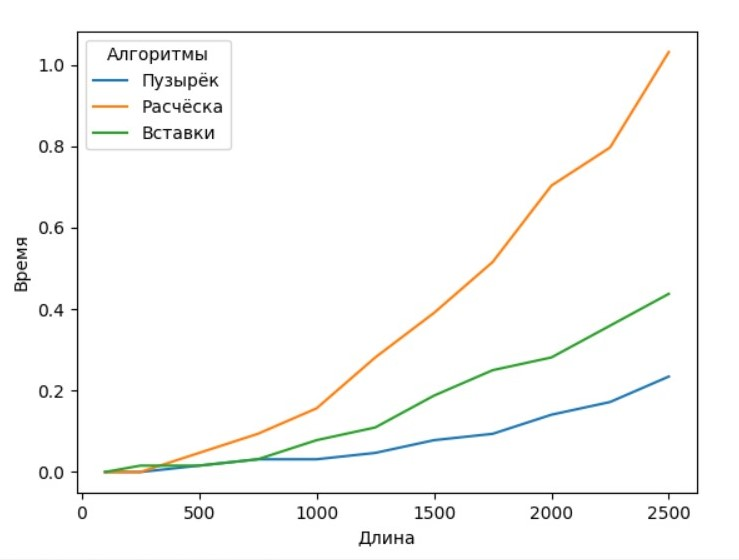
\includegraphics[scale=0.5]{res_graph}}
	\caption{График зависимости времени свёртки от размерности матрицы}
\end{figure}

\section{Вывод}
В результате эксперимента было получено, что на квадратных матрицах размерами от 100 на 100 до 2000 на 2000 распаралеливание позволяет добиться практически шестикратного (5,931) ускорения при использовании 64 потоков. Также можно заметить, что при увеличении количества потоков в два раза, скорость выполнения уменьшается в среднем в два раза относительно предыдущей. В результате можно сделать вывод о том, что использование параллельного программированние позволяет значительно ускорить работу некоторых алгоритмов.